\tikzset{%
	every neuron/.style={
		circle,
		draw,
		minimum size=1cm
	},
	neuron missing/.style={
		draw=none, 
		scale=4,
		text height=0.333cm,
		execute at begin node=\color{black}$\vdots$
	},
}

\begin{figure}[t]
	\centering
	\resizebox{0.6\textwidth}{!}{
		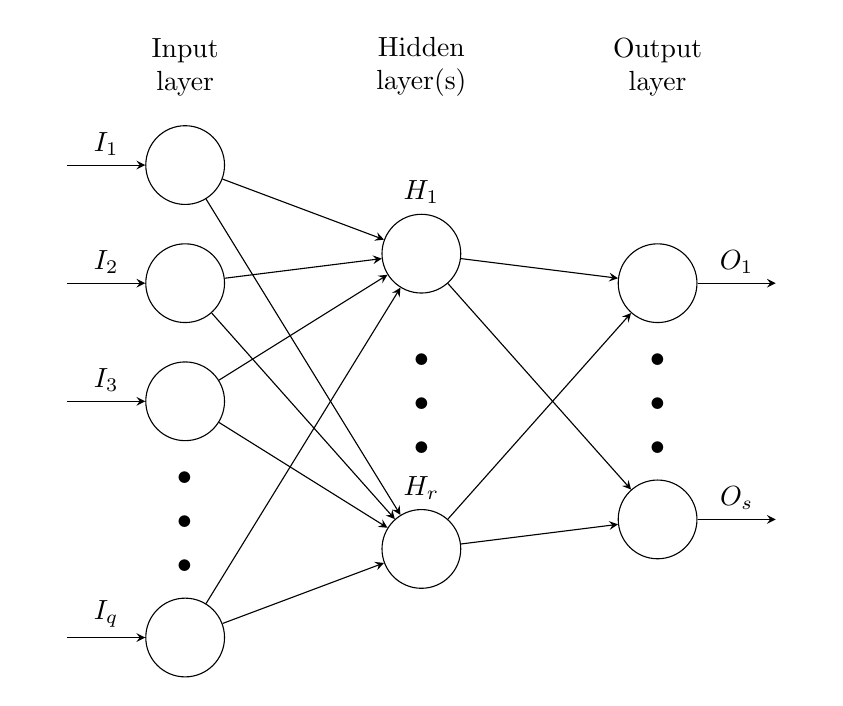
\begin{tikzpicture}[x=1.5cm, y=1.5cm, >=stealth]
			% Input neurons
			\foreach \m/\l [count=\y] in {1,2,3,missing,4}
			  \node [every neuron/.try, neuron \m/.try] (input-\m) at (0,2.5-\y) {};
			% Hidden neurons
			\foreach \m [count=\y] in {1,missing,2}
			  \node [every neuron/.try, neuron \m/.try ] (hidden-\m) at (2,2-\y*1.25) {};
			% Output neurons
			\foreach \m [count=\y] in {1,missing,2}
			  \node [every neuron/.try, neuron \m/.try ] (output-\m) at (4,1.5-\y) {};
			% Input labels
			\foreach \l [count=\i] in {1,2,3,q}
			  \draw [<-] (input-\i) -- ++(-1,0)
			    node [above, midway] {$I_\l$};
			% Hidden neuron labels
			\foreach \l [count=\i] in {1,r}
			  \node [above] at (hidden-\i.north) {$H_\l$};
			% Out arrows with labels
			\foreach \l [count=\i] in {1,s}
			  \draw [->] (output-\i) -- ++(1,0)
			    node [above, midway] {$O_\l$};
			% Input to hidden arrows
			\foreach \i in {1,...,4}
			  \foreach \j in {1,...,2}
			    \draw [->] (input-\i) -- (hidden-\j);
			% Hidden to output arrows
			\foreach \i in {1,...,2}
			  \foreach \j in {1,...,2}
			    \draw [->] (hidden-\i) -- (output-\j);
			% Layer labels
			\node [align=center, above] at (0,2) {Input \\ layer};
			\node [align=center, above] at (2,2) {Hidden \\ layer(s)};
			\node [align=center, above] at (4,2) {Output \\ layer};
		\end{tikzpicture}
	}
	\caption[Artificial Neural Networks]{A Visualization of how neurons interact within an artificial neural network. In this example, the network has 3 layers: An input layer, a hidden layer, and an output layer. The input layer consists of $q$ neurons, each having one input value. Each of these inputs neurons are connected to each of the $r$ neuron in the hidden layer. Each neuron in the hidden layer is also connected to each neuron in the output layer. Finally, the output layer contains $s$ neurons and returns $s$ output values.}\label{fig:background-neuralnet}
\end{figure}